%
% Niniejszy plik stanowi przykład formatowania pracy magisterskiej na
% Wydziale MIM UW.  Szkielet użytych poleceń można wykorzystywać do
% woli, np. formatujac wlasna prace.
%
% Zawartosc merytoryczna stanowi oryginalnosiagniecie
% naukowosciowe Marcina Wolinskiego.  Wszelkie prawa zastrzeżone.
%
% Copyright (c) 2001 by Marcin Woliński <M.Wolinski@gust.org.pl>
% Poprawki spowodowane zmianami przepisów - Marcin Szczuka, 1.10.2004
% Poprawki spowodowane zmianami przepisow i ujednolicenie
% - Seweryn Karłowicz, 05.05.2006
% Dodanie wielu autorów i tłumaczenia na angielski - Kuba Pochrybniak, 29.11.2016

% dodaj opcję [licencjacka] dla pracy licencjackiej
% dodaj opcję [en] dla wersji angielskiej (mogą być obie: [licencjacka,en])
\documentclass[en]{pracamgr}

% Code listings
\usepackage{listings}
\usepackage{xcolor}
\usepackage{amsmath}
% Diagrams
\usepackage{tikz}
\usetikzlibrary{calc,positioning,arrows.meta,shapes,fit,backgrounds}

\usepackage{pgfplots}
\usepgfplotslibrary{groupplots}
\pgfplotsset{width=10cm, compat=1.9}
\usepackage{float}

\definecolor{codegreen}{rgb}{0,0.6,0}
\definecolor{codegray}{rgb}{0.5,0.5,0.5}
\definecolor{codepurple}{rgb}{0.58,0,0.82}
\definecolor{backcolour}{rgb}{1,1,1}

\lstdefinestyle{mystyle}{
    backgroundcolor=\color{backcolour},
    commentstyle=\color{codegreen},
    keywordstyle=\color{magenta},
    numberstyle=\tiny\color{codegray},
    stringstyle=\color{codepurple},
    basicstyle=\ttfamily\footnotesize,
    breakatwhitespace=false,
    breaklines=true,
    captionpos=b,
    keepspaces=true,
    numbers=left,
    numbersep=5pt,
    showspaces=false,
    showstringspaces=false,
    showtabs=false,
    tabsize=2
}
\lstset{basicstyle = \ttfamily, style=mystyle, frame=single, numbers=none, columns=fullflexible, upquote=true}
% End code listings

% Hrefs
\usepackage[colorlinks]{hyperref}
\hypersetup{
    linkcolor=red,
    citecolor=blue,
    urlcolor=magenta,
}
\usepackage{caption} % makes clicking figure \ref navigate to the top of the figure instead of the caption
% End hrefs

\usepackage[dateabbrev=false,date=iso,urldate=iso]{biblatex}
\usepackage{csquotes}

\addbibresource{references.bib}

% Dane magistranta:
\autor{Krzysztof Małysa}{394442}

\title{Multi-process sandbox for unprivileged users on Linux}
\titlepl{Sandbox wielu procesów dla nieuprzywilejowanych użytkowników systemu Linux}

%\tytulang{An implementation of a difference blabalizer based on the theory of $\sigma$ -- $\rho$ phetors}

%kierunek:
% - matematyka, informacyka, ...
% - Mathematics, Computer Science, ...
\kierunek{Computer Science}

% informatyka - nie okreslamy zakresu (opcja zakomentowana)
% matematyka - zakres moze pozostac nieokreslony,
% a jesli ma byc okreslony dla pracy mgr,
% to przyjmuje jedna z wartosci:
% {metod matematycznych w finansach}
% {metod matematycznych w ubezpieczeniach}
% {matematyki stosowanej}
% {nauczania matematyki}
% Dla pracy licencjackiej mamy natomiast
% mozliwosc wpisania takiej wartosci zakresu:
% {Jednoczesnych Studiow Ekonomiczno--Matematycznych}

% \zakres{Tu wpisac, jesli trzeba, jedna z opcji podanych wyzej}

% Praca wykonana pod kierunkiem:
% (podać tytuł/stopień imię i nazwisko opiekuna
% Instytut
% ew. Wydział ew. Uczelnia (jeżeli nie MIM UW))
\opiekun{dr Janina Mincer-Daszkiewicz\\Institute of Informatics}

% miesiąc i~rok:
\date{December 2022}
% \date{TODO}

%Podać dziedzinę wg klasyfikacji Socrates-Erasmus:
\dziedzina{
%11.0 Matematyka, Informatyka:\\
%11.1 Matematyka\\
%11.2 Statystyka\\
11.3 Informatics, Computer Science\\
%11.4 Sztuczna inteligencja\\
%11.5 Nauki aktuarialne\\
%11.9 Inne nauki matematyczne i informatyczne
}

%Klasyfikacja tematyczna wedlug AMS (matematyka) lub ACM (informatyka)
\klasyfikacja{Security and privacy -- Systems security -- Operating systems security}

% Słowa kluczowe:
\keywords{sandboxing, security, Linux, secure execution, arbitrary code execution, judging system, } %, capabilities, cgroups, user namespace, PID namespace, mount namespace, rlimit, seccomp, ptrace}

% Tu jest dobre miejsce na Twoje własne makra i~środowiska:
% \newtheorem{defi}{Definicja}[section]

% koniec definicji

\begin{document}
\renewcommand\textfraction{0}

\maketitle

%tu idzie streszczenie na strone poczatkowa
\begin{abstract}
TODO
\iffalse
We introduce a new sandbox for unprivileged Linux users that requires no kernel modifications. It takes advantage of several Linux mechanisms used elsewhere --- cgroups, namespaces, ptrace and seccomp among others. The sandbox was optimized to run dozens of untrusted programs in a sequence with minimal overhead while preserving the safety. It is capable of running both multi-threaded and multi-process programs. It is able to record the peek memory usage and CPU execution time of multithreaded program, alas these statistics are unavailable for multi-process programs.
We describe the encountered limitation and challenges around enforcing safety and collecting statistics. Further, we examine its ability to run complex multi-process programs like C++ compiler and the overhead when running a series of short-running programs.
\fi
\end{abstract}

\tableofcontents
%\listoffigures
%\listoftables

\chapter{Introduction}\label{chapter:introduction}

\section{Background}

Secure execution environments are commonplace these days, from containers and virtual machines on servers to sandboxes on laptop and smartphones --- most of which run on Linux. They are used to securely execute untrusted code, as well as trusted programs to prevent damage escalation in the event of unknown vulnerabilities. Their key features are isolation, limiting resource usage, and accounting for resource consumption.

The features of Linux allow the creation of simple yet effective and efficient secure environments. They work at application runtime, so in most cases existing software does not need to be adapted to use them. This makes them easily applicable, and explains why their adoption is growing.

In this thesis, the most important application of sandboxing are online judge systems. Online judge systems have beneficial role in programming education and competitive programming. They allow testing user-provided solution to a specific problem. The solution is run on a predefined test cases in order to check if it is valid. In such platforms isolating the compilation and running of the solution is essential to provide security and robustness of the platform itself.

Historically, isolation techniques evolved together with the online judge platforms. The most primitive (yet insecure) was usage of \texttt{chroot(2)} \cite{prevelakis2001sandboxing} to restrict access to part of the filesystem. To increase isolation virtual machines were used \cite{5635141}. Later, containerization became a new way to provide isolation \cite{marevs2012new, SPACEK20151665}.

Online education platforms greatly facilitate teaching and learning programming. They provide quick feedback on the correctness of the code the user submits. They are used in schools and universities and provide great learning opportunities for all.

Moreover, a versatile sandbox has applications outside online judging platforms. For example, it can be used to sanitize compiling a PDF form \LaTeX~sources or for safe execution of untrusted server-side scripts in web applications.

\section{Goal of the thesis}

The goal of the thesis is to design, implement and integrate a new sandbox for the Sim project \cite{sim_project}. The Sim project is an online platform for preparing people for and carrying out algorithmic contests. The project started in 2012 and is developed by me since the beginning. It is used at the XIII High School in Szczecin and programming camps to teach young people programming and algorithms. It has an online judge with a sandbox specially developed for this use case. Over the years the sandbox became a limitation. It only allows running a single-threaded statically linked executable of programs written in C, C++ or Pascal. The new sandbox will allow supporting more programming languages and improve security of the solution compilation stage.

\subsection{Requirements}

The new sandbox needs to be optimized for running short-running programs as well as have minimal runtime overhead. Most of the test cases the solution is run on are small and solution completes them in less than 10ms. The goal is to allow hundreds of such sort-running runs per second, hence optimizing for short-running programs is important. However, minimizing overhead of the sandbox during the run is also important i.e. if the program runs X ms normally, the objective is that the program inside the new sandbox will also run approximately X ms.

The new sandbox needs to be versatile. It will be used to secure the compilation of the solutions as well as running of the solutions. Compilation is a complicated process that involves parsing, translating, optimizing and linking the final program. For languages like C, C++ and Rust it involves running several executables in coordination e.g. compiler and linker i.e. more than one process at a moment --- the sandbox needs to support that.

Sandboxing needs to have a low overhead. Apart from small test where solution runs quickly (a matter of milliseconds), almost always the solution is run on big test cases, where it may need several seconds for it to solve the problem. Increasing this time as little as possible while the solution is running inside the sandbox is one of the primary objectives.

It often requires running several executables e.g. compiler and linker, so allowing a single process inside sandbox is not enough. Sandboxing solution is simpler, because it is a single process. But since it is often short-running, the overhead needs to be minimal.

The sandbox needs to allow limiting resources. Real time, CPU time, memory -- these need to be limited not only for the robustness of the platform, but specific problems require different limits. The goal of some problems is to solve it with very restricted memory e.g. find a missing integer in a random permutation of integers $1, \ldots, n$ without one element, but in constant memory.

The sandbox needs to account resource usage. For every test, the user is presented with consumed memory and CPU time by their solution. The sandbox needs to provide this information.

The last requirement is the sandbox will not require any privileges. There is a tool called Sip \cite{sip} for preparing the problem packages for the Sim platform. One of the purposes of the tool is to run the solutions inside the same secure environment as on the Sim platform. The user should not need any privileges to run this tool, so the sandbox should not require them either.

\subsection{Existing solutions}

Approaches to form a secure execution environments differ. One of them is virtualization or emulation e.g. QEMU \cite{qemu_website} and KVM \cite{kvm_website}, VirtualBox \cite{virtualbox_website}, VMWare Workstation \cite{vmware_workstation_website}. Although powerful and effective, they come with an enormous overhead i.e. booting up an entire operating system. Moreover, emulation noticeably slows down the runtime of an emulated application, rendering such solutions inapplicable.

Containers provide much lower overhead: setup of an order of milliseconds and negligible runtime overhead. But, Docker \cite{Merkel:2014:DLL:2600239.2600241}, LXC \cite{conf/cisis/BeserraMEBSF15} require root privileges to create a container. systemd-nspawn \cite{systemd_nspawn} requires root privileges to run.

Rootless are containers \cite{rootless_containers_rs} that can be created and run by an unprivileged user are the almost perfect solution to the problem. They provide almost all of the functionality of the normal containers but without the need to engage a privileged user. However, they often use setuid binaries and that is undesirable \cite{podman_rootless_containers_presentation}. Also they are not optimized to run sequences of short-running programs. In this thesis we will create a sandbox that uses the same techniques as rootless containers but will be optimized for running sequences of short-running programs.

% \section{Scope}

% The sandbox is implemented in C++ and runs only on Linux. The implementation was tested on x86\_64 but should also work on x86 or arm64, due to no architecture specific parts. Only seccomp filters may need to be adapted for other architectures, but the sandbox itself uses user-provided seccomp filters so it should work out of the box.

% The sandbox uses linux namespaces to isolate the sandboxed program and cgroups to limit resources and provide resource usage accounting.

% A sandbox client in Rust language would be beneficial for the broader adoption of the sandbox, but is intentionally out of scope of this thesis.

\section{Structure of the Thesis}

Chapter \ref{chapter:literature_overview} contains overview of sandboxing techniques and existing implementations and comparative analysis of them. Details of design and architecture are described in chapter \ref{chapter:design}. Implementation is described in \ref{chapter:implementation}. Chapter \ref{chapter:performance} contains performance evaluation of the final implementation and impact of some optimizations. Later, in chapter \ref{chapter:use_cases} use cases and applications are discussed. Chapter \ref{chapter:integration} details integration with online judge and challenges involved. In chapter \ref{chapter:future_work} future work and opportunities are discussed. Finally, chapter \ref{chapter:conclusion} contains the conclusion.

\chapter{Literature overview}\label{chapter:literature_overview}

\section{Overview of Sandboxing Techniques}

During the first programming competitions, the human judges manually read and verified the source code of the contestants' solutions \cite{tochev2010validating}. Over time this became infeasible and gave birth to automatic judge systems.

To prevent people from interfering with the normal workflow of the competition e.g. Denial of Service Attack by exhausting memory resources, the automatic judge systems need a secure way to compile and execute a contest's solution. This is where sandboxes come into place.

First sandboxes required modification of the OS kernel \cite{provos2003improving, garfinkel2004janus, garfinkel2004ostia, jana2011txbox, li2014minibox}. While they had little run-time overhead, some of them were limited to single-threaded applications \cite{merry2009using}.

Later, as support for process tracing matured, \texttt{ptrace}-based sandboxes arose \cite{marevs2007perspectives, kolstad2009infrastructure, kim2013practical}. The problem with those solutions is the overhead that varies from around 75\% \cite{merry2010performance} to 160\% \cite{marevs2012new} for syscall-intensive programs. This overhead however, does not affect programming contest fairness much \cite{marevs2011fairness}. Supporting multi-threaded and multi-process programs while using \texttt{ptrace} is tricky, but possible \cite{kim2013practical}, because of Time of Check/Time of Use (TOCTOU) problem \cite{cwe_toctou}. \texttt{ptrace}-based sandbox needs to inspect syscall arguments. To do so it has to read them, but the multi-threaded or multi-process program can change the indirect argument after the reading but before the kernel uses the argument. This creates a dangerous race condition that has to be addressed.

Finally, after the kernel support for containerization materialized, namespace and cgroup based sandboxes came into place \cite{marevs2012new, netblue30/firejail, raknes2016nsroot, google/nsjail, flatpak, SPACEK20151665}. Contrary to ptrace-based sandboxes, namespace-based sandboxes have negligible runtime overhead \cite{marevs2012new}. Moreover, they don't require modifications of the Linux kernel and work on major Linux distributions out of the box.

\section{Existing Implementations}

\subsection{Modifying OS kernel}

\subsubsection{Systrace}

Systrace \cite{provos2003improving} intercepts all system calls in the kernel. It then decides if the syscall is safe by first checking a static list of safe syscalls. This step exists to reduce sandboxing performance overhead. If the syscall is not on the list, Systrace consults user space for a decision.

The system avoids TOCTOU problem \cite{cwe_toctou} by copying syscall arguments to kernel memory before asking user space for a decision.

\subsubsection{Janus}
Janus \cite{garfinkel2004janus} adds a module to extend Linux \texttt{ptrace} API. Policies are defined using configuration files. By default all syscalls are denied. The configuration directive refers to the policy module that provides the logic for deciding whether to allow a particular system call or not. For example, \texttt{path} module could be used to restrict IO on certain file paths.

\subsubsection{Ostia}
Ostia \cite{garfinkel2004ostia} instead of filtering system calls it delegates them to an external agent that performs syscalls on behalf of the sandboxed process. Authors emphasize that such architecture simplifies the system and protects from TOCTOU problems \cite{cwe_toctou}.

Ostia is implemented as two components: a small kernel module and a user space part. The module intercepts the syscall and copies its arguments via IPC link to the user space agent. The agent decides whether the call should be allowed, executes it and returns the results back over the IPC link. Worth noting is that not all syscalls have to delegated~---~some can be always allowed while others always denied.

\subsubsection{TxBox}
TxBox \cite{jana2011txbox} introduces system-level transaction support. Impact of the untrusted insecure code is limited by rolling back the system state after the execution. This provides strong isolation and works with arbitrary executables but requires significant out-of-tree patches of the OS kernel.

\subsubsection{MiniBox}
MiniBox \cite{li2014minibox} is a two-way sandbox that protects operating system from the application as well as application from the operating system. A modified version of TrustVisor \cite{mccune2010trustvisor} hypervisor runs OS and sandboxed application separately in a Mutually Isolated Execution Environment. The hypervisor is the only communication channel between the isolated application and the regular OS. This way application is protected from the malicious operating system. To protect the OS from the application, MiniBox uses Software Fault Isolation techniques from NaCl \cite{yee2010native}.

\subsubsection{SACO sandbox}

South African Computer Olympiad (SACO) sandbox \cite{merry2009using} inserts a custom kernel module that hooks up to Linux Security Module infrastructure. Although it has negligible time and memory overhead, it only supports single-threaded programs.

\subsection{\texttt{ptrace}-based}

\subsubsection{MO sandbox}
MO sandbox \cite{marevs2007perspectives, kolstad2009infrastructure} allows only single-threaded programs. It simply inspects arguments using \texttt{ptrace} and uses \texttt{setrlimit} \cite{man_getrlimit_setrlimit_prlimit} to limit resources. It is used by USA Computer Olympiad (USACO).

\subsubsection{MBOX}
MBOX \cite{kim2013practical} requires no superuser privileges. It makes use of seccomp BPF system call filtering to restrict allowed syscalls. BPF filtering is effective only for non-indirect arguments. To address this issue, the installed BPF filter notifies the \texttt{ptrace} monitoring process if further argument inspection is necessary to make a decision. To avoid TOCTOU problem \cite{cwe_toctou}, the MBOX allocates a read-only page to which it copies the indirect arguments before inspecting them and rewrites the syscall to use the rewritten arguments. The copied arguments are protected against modification because changing page access permissions is impossible without a syscall.

\subsection{Using Linux namespaces}

\subsubsection{Firejail}
Firejail \cite{netblue30/firejail} uses seccomp BPF system call filtering and mount namespaces to restrict filesystem access. Similarly it uses process namespaces to limit view of running processes and network namespaces to restrict access to network devices. However, Firejail uses a \texttt{setuid} \cite{man_setuid} helper binary to achieve that. It allows resource limiting through \texttt{prlimit} \cite{man_getrlimit_setrlimit_prlimit}.

\subsubsection{nsjail} \label{subsubsection:nsjail}
nsjail \cite{google/nsjail} uses Linux namespaces, seccomp BPF system call filtering, \texttt{setrlimit} \cite{man_getrlimit_setrlimit_prlimit} and cgroups to limit resources. It does not require superuser privileges. However, it is not optimized for running short-running programs. Also, it does not provide statistics of the run.

\subsubsection{nsroot}
nsroot \cite{raknes2016nsroot} does not support resource limiting. It only makes use of Linux namespaces to restrict view of the file system, IPC and network devices.

\subsubsection{Flatpak}
Flatpak \cite{flatpak}, previously xdg-app, is a software packaging and sandboxing tool. Internally, it uses Bubblewrap sandbox. The Bubblewrap \cite{bubblewrap} is a \texttt{setuid} \cite{man_setuid} program that uses Linux namespaces and seccomp filters.

\subsubsection{New Contest Sandbox}
New Contest Sandbox \cite{marevs2012new} uses Linux namespaces and cgroups but not seccomp filters. It is used by Moe modular contest system (2012) \cite{marevs2012new}. Linux namespaces and cgroups have negligible overhead compared to \texttt{ptrace}.

\subsubsection{APAC}
APAC (Automatic Programming Assignment Checker) \cite{SPACEK20151665} uses Docker for sandboxing. It sets up a container for each run. Docker uses runC under the hood. While runtime overhead of Docker is low, the setup phase is primary source of overhead for short-running programs.

\subsubsection{runC}
runC \cite{cochak2021runc} uses the same features of Linux kernel as nsjail. However, configuration is stored as files instead of passed as command-line arguments. It has a special \texttt{rootless} mode which does not require superuser privileges. Given all of the above however, it is not optimized for running short-running programs. runC is used internally by Docker.

\subsection{Other}

\subsubsection{Google Native Client}
Native Client (NaCl) \cite{yee2010native} uses static analysis and Software Fault Isolation. After the static analysis, the program runs at native speed but requires recompilation with special compiler and libraries. NaCl only works for x86 architecture.

\section{Conclusion}

Many sandboxing solutions exist. From all of the above, closest to our requirements is nsjail (see Section \ref{subsubsection:nsjail}). However, it is not optimised for running short-running programs. In fact, none of the above solutions is optimised to run hundreds of short-running programs per second.

Considering the similarities of nsjail and our solution, in the performance analysis we will compare our sandbox to nsjail sandbox.

% Overhead caused by context switches can be minimized by restricting the process or group of processes to a separate cpuset \cite{merry2010performance}.

\chapter{Design and Architecture}\label{chapter:design}

\section{Client-server architecture}

From the start the sandbox was based on the client-server architecture. This was the choice to minimize process cloning overhead \cite{redis-latency-generated-by-fork}, since it is a costly operation and happens for every sandboxing request. fork/clone needs to clone the whole address space of the process and the client process could have a large address space. Server process that is executed from a separate executable has a minimal required address space size therefore the cloning overhead is minimal for every request. Moreover, this architecture easily and safely allows sharing as much work as possible between the sandboxing requests which is the key to low overhead of running short-running programs.

The client spawns the sandboxing server and sends sandboxing requests via UNIX domain socket to the server. The request contains executable, arguments, namespace configuration, resource limits, seccomp BPF filters and a pipe through which the result will be sent back.

At startup, the server creates cgroup hierarchy and some namespaces so that they won't have to be created later or their creation will be faster. Other utilities are also setup here to do it once instead of for every request. Then it starts accepting requests.

\subsection{Sandboxing request handling}

For each request, the server process (aka supervisor) spawns the PID 1 process of the new PID namespace. Then the init process setups namespaces and some of the resource limits. Finally the PID 1 process spawns the tracee process that finishes configuration and executes the requested executable. So for each sandboxing request we spawn exactly 2 processes. The PID 1 process is necessary for a couple of reasons:
\begin{itemize}
    \item It reaps the zombie processes in the tracee PID namespace.
    \item It allows locking mount-points in the mount namespace. The tracee process is spawned in a new user and mount namespace. Mounts are performed by the PID 1 process, therefore all mounts become locked together and cannot be individually unmounted by the tracee \cite{man_mount_namespaces}. These mounts cannot be performed by the supervisor process instead, because it would alter the mount namespace for subsequent requests.
    \item Inside a PID namespace, sending signals to the PID 1 process is allowed only for signals that the PID 1 process installed signal handler for. This could change the behavior for some programs, therefore a helper PID 1 process is needed.
\end{itemize}

\section{Cgroups}

The server gains write access to cgroup hierarchy by being executed through \texttt{systemd-run -{}-user -{}-scope -{}-property=Delegate=yes -{}-collect}. It enables \texttt{pid}, \texttt{memory}, and \texttt{cpu} controllers for the below subgroups.

The server process creates at startup the cgroup v2 hierarchy that looks as follows:
\begin{itemize}
    \item \texttt{/supervisor} --- cgroup of the supervisor process,
    \item \texttt{/pid1} --- cgroup of the pid1 process,
    \item \texttt{/tracee} --- cgroup of the tracee processes.
\end{itemize}
After creation of the hierarchy it places the supervisor process in its cgroup. Subsequent processes are placed in their cgroups by making use of \texttt{CLONE\_INTO\_CGROUP} flag.
\newline
\texttt{/tracee} cgroup allows:
\begin{itemize}
    \item Killing all tracee processes by writing 1 to \texttt{/tracee/cgroup.kill} file.
    \item Reading CPU user and CPU system time via \texttt{/tracee/cpu.stat} file.
    \item Reading peak memory usage via \texttt{/tracee/memory.peak} file.
    \item Setting process/tread number limit by writing \texttt{/tracee/pids.max}.
    \item Setting memory hard limit by writing \texttt{/tracee/memory.max}.
    \item Setting CPU usage limit by writing \texttt{/tracee/cpu.max}.
    \item Disabling PSI accounting to reduce the sandboxing overhead by writing 0 to \texttt{/tracee/cgroup.pressure} file.
\end{itemize}
\texttt{/tracee} cgroup needs to be deleted and recreated after each request to reset \texttt{/tracee/cpu.stat} and \texttt{/tracee/memory.peak} files.

\section{Linux namespaces}

Linux allows unprivileged users to create user namespaces only. However, after entering a new user namespace the process gains all privileges inside the namespace and can create other namespaces.
\newline
The supervisor process creates the following namespaces:
\begin{itemize}
    \item user namespace --- in order to create other namespaces and hide user ID and group ID,
    \item cgroup namespace --- to allow mounting detached cgroups v2 hierarchy,
    \item mount namespace --- to allow mounting detached cgroups v2 hierarchy,
    \item network namespace --- to disconnect every tracee from network devices, done once, as it is costly,
    \item IPC namespace --- to isolate every tracee from other processes' IPC, done once, for optimization,
    \item UTS namespace --- to isolate every tracee from host's hostname, done once, for optimization,
    \item time namespace --- to isolate every tracee from host's time namespace, done once, for optimization.
\end{itemize}
The pid1 process creates the following namespaces:
\begin{itemize}
    \item user namespace --- in order to create other namespaces and hide user ID and group ID,
    \item mount namespace --- to allow mounting requested mount-point hierarchy,
    \item PID namespace --- to isolate tracee from accessing other processes.
\end{itemize}
The tracee process creates the following namespaces:
\begin{itemize}
    \item user namespace --- in order to create other namespaces and hide user ID and group ID and lock the mount tree,
    \item mount namespace --- in lock the mount tree created by pid1.
\end{itemize}

\section{Inter-process communication}

The client sends requests via UNIX domain socket to the supervisor process. The results are sent via a pipe attached to the request. The pipe is attached to the request as a file descriptor using \texttt{SCM\_RIGHTS} control message \cite{man_unix}.

The supervisor, pid1 and tracee process communicate via shared anonymous memory page. Such communication requires no syscalls, is fast and reliable. This page is automatically unmapped upon \texttt{execveat} syscall \cite{man_execveat} in the tracee process, so it is protected from the tracee access.

\section{Capabilities}

The supervisor process drops all capabilities, sets securebits and \texttt{NO\_NEW\_PRIVS} flag. This ensures minimal possible capabilities in its and ancestor user namespace and prevents gaining any new privileges.

\section{Hardening}

The pid1 process, after spawning the tracee enters a new cgroup namespace to limit view of other namespaces i.e. if the tracee somehow takes control of the pid1 process, it will not be able to raise its PID and memory limit. Moreover a seccomp filter is installed to limit allowed syscalls only to those needed for reaping the orphaned zombie process, managing time limits and exiting upon tracee death.

\chapter{Implementation}\label{chapter:implementation}

\chapter{Performance Evaluation}\label{chapter:performance}

\chapter{Use Cases and Applications}\label{chapter:use_cases}

\chapter{Integration with Online Judge}\label{chapter:integration}

\chapter{Future work and Opportunities}\label{chapter:future_work}

\chapter{Conclusion}\label{chapter:conclusion}

% Is to create a sandbox optimized for an online judge i.e. optimized for running the same program multiple times with different input. Also the sandbox has to be capable enough to allow running a compiler. However the below assumptions must be met:
% \begin{itemize}
%     \item The system is running with cgroup v2
%     \item The system is running with systemd
%     \item Unprivileged user namespaces are enabled
% \end{itemize}
% The sandbox has to provide execution statistics:
% \begin{itemize}
%     \item Memory used
%     \item Execution CPU time
%     \item Execution real time
% \end{itemize}
% with the following limits and isolation:
% \begin{itemize}
%     \item Real time limit
%     \item CPU time limit for single process programs
%     \item Memory limit
%     \item Stack memory limit
%     \item Process limit
%     \item Filesystem isolation with allowing bindings
%     \item Visible processes isolation
%     \item Visible users isolation
%     \item Visible IPC isolation
%     \item Network isolation
%     \item Hostname isolation
% \end{itemize}

% \section{Structure of the thesis}

% Chapter \ref{chapter:kernel_features} contains brief summary of the Linux kernel features employed by the sandbox. Chapter \ref{chapter:sandbox_design} describes the sandbox and its design. In chapter \ref{chapter:comparison_with_rootless_containers} comparison with the rootless containers is described.

% \chapter{Kernel features}\label{chapter:kernel_features}

% % \chapter{Design considerations}\label{chapter:design_considerations}

% \chapter{Sandbox design}\label{chapter:sandbox_design}

% \chapter{Comparison with rootless containers}\label{chapter:comparison_with_rootless_containers}

\iffalse
TODO

\section{Assumptions}

The primary assumption is that the validation and enforcement during the interaction of an untrusted program and the Linux kernel is enough to prevent the program from doing anything unwanted. Thus sanitization of all syscalls either directly (using \texttt{ptrace} and \texttt{seccomp}) or indirectly (using capabilities, cgroups, namespaces e.g. mount namespaces, and limits e.g. \texttt{prlimit()}). Thereby executing the program while no syscalls are invoked is considered safe. In general however, this is not true, e.g. \texttt{io\_uring} can be used to ''call syscalls'' without actually executing any syscall \cite{io_uring_paper, io_uring_kernel_recipes, lwn_io_uring, lwn_io_uring_2}. Another example is writing to memory mapped file just by writing to the memory region where the file is mapped to. Such dangerous situations need to be prevented by properly forbidding or sanitizing syscalls that are necessary for such situations to happen i.e. preventing \texttt{io\_uring} syscalls and forbidding mapping of the unwanted files.

% The objective of this project is to create safe and efficient sandbox to execute short running untrusted programs, as well as complex programs e.g. compiler of a C++ program. All done with robust isolation and minimal overhead (the order of milliseconds).

% The primary use case is an online judge whose job is to
% \begin{itemize}
%     \item compile user-provided source code
%     \item run it several times (even hundreds) with different inputs
%     \item verify the output correctness usually by running another program
% \end{itemize}
% All of these tasks require at least ensuring that
% \begin{itemize}
%     \item real time is limited
%     \item CPU time is limited
%     \item memory is limited
%     \item disk space is limited
%     \item file access is isolated
%     \item network is isolated or disabled
% \end{itemize}
% Also statistics about the executed program are required
% \begin{itemize}
%     \item real time used
%     \item CPU time used
%     \item peek memory usage
% \end{itemize}
% All of that is to be done as an unprivileged user.

% Such combination (especially minimal overhead and recording the peek memory usage) is very uncommon e.g. Firejail (TODO: reference) does not provide memory statistics. LXC (TODO: reference) and Docker require privileges to create a container. Thereby, the listed constraints require a new solution.

% In the chapter \ref{chapter:linux_mechanism}, we describe the Linux kernel mechanisms used in the project and . Design of the sandbox is described in chapter \ref{chapter:design} along with security considerations and decisions made in the process along with the encountered limitations such as inability to record the peak memory usage and total CPU time when more that one process is running. The chapter \ref{chapter:evaluation} contains performance measurements of the sandbox and evaluation of ability to run complex programs like C++ compiler or \LaTeX engine.

\chapter{Useful Linux kernel mechanisms} \label{chapter:linux_mechanism}

TODO

\section{User namespaces}
TODO

\section{PID namespaces}
TODO

\section{Mount namespaces}

Mount namespaces allow for isolation of mounts i.e. process in one namespace can modify its mount list without affecting others' mount lists, or affecting or being affected by others in a controlled manner thanks to the Shared Subtrees feature of the Linux kernel \cite{shared_subtree}.

\subsection{Terminology}

The most typical use case of \texttt{mount} is mounting a filesystem at some location in a filesystem e.g. mounting home directory: \texttt{mount /dev/sda2 /home/user} or mounting the temporary filesystem at \texttt{/tmp}: \texttt{mount -t tmpfs tmpfs /tmp}. Filesystem can be mounted at multiple locations e.g. \texttt{mount /dev/sda2 /a \&\& mount /dev/sda2 /b}. Such location is called a \textbf{mount point}. As it will be explained later, a single \textbf{mount} has a single mount points. But a single \texttt{mount} operation may result in more than one mounts.

List of all mounts of a mount namespace of a process with PID \texttt{[pid]} can be examined via file \texttt{/proc/[pid]/mountinfo}.

\paragraph{Mount} is a result of a \texttt{mount} operation and is a filesystem that is accessible at a specified location called a \texttt{mount point}.

\paragraph{Mount point} is a location where mount in attached.

\paragraph{Propagation type} affects how mounts that happen directly under that mount are propagated to other members of the \texttt{peer group} and its slave peer groups. It can be one of:
\begin{itemize}
    \item \texttt{shared} Its peer group can have any size and mount events propagate to other members and from other members of the peer group.
    \item \texttt{slave} Its peer group has only one member --- itself and has a master peer group. Mount events propagate from the master peer group, but not to the master peer group.
    \item \texttt{slave \& shared} Its peer group can have any size and has a master peer group. Mount events propagate between members of the slave \& shared peer group but not to the master peer group. Mount events from the master peer group propagate to all members of the slave \& shared peer group.
    \item \texttt{private} Its peer group has only one member --- itself. No mount events propagate from this peer group to another and vice versa.
    \item \texttt{unbindable} Same as \texttt{private}, but bind mounts with source inside this mount are forbidden.
\end{itemize}

\paragraph{Peer group} is a group of mounts that propagate mounts between one another.

These notions are best illustrated in an example. First we mount \texttt{tmpfs} at \texttt{/mnt} and make its propagation type \texttt{shared}, later we examine the mount list after this operation.
\begin{lstlisting}
# mount -t tmpfs tmpfs /mnt --make-shared
# cat /proc/self/mountinfo | grep '/mnt' | sed 's/ - .*//'
619 27 0:69 / /mnt rw,relatime shared:274
\end{lstlisting}
Now we create a \texttt{/tmp/mnt} and bind mount there the \texttt{/mnt}.
\begin{lstlisting}
# mkdir /tmp/mnt
# mount --bind /mnt /tmp/mnt
# cat /proc/self/mountinfo | grep '/mnt' | sed 's/ - .*//'
619 27 0:69 / /mnt rw,relatime shared:274
773 39 0:69 / /tmp/mnt rw,relatime shared:274
\end{lstlisting}
We see that both of these mounts have \texttt{shared:274} --- it means that the mount has propagation type \texttt{shared} and \texttt{274} is the id of the peer group. So both mounts are in the same peer group.
Apart from the fact that these mount points have the same filesystem underneath (because of the bind mount):
\begin{lstlisting}
# ls /mnt
# ls /tmp/mnt
# touch /mnt/a
# touch /tmp/mnt/b
# ls /mnt
a  b
# ls /tmp/mnt
a  b
\end{lstlisting}
They also propagate mount events between them (because of the propagation type \texttt{shared}):
\begin{lstlisting}
# mkdir /mnt/c
# mount -t tmpfs tmpfs /mnt/c
# cat /proc/self/mountinfo | grep '/mnt' | sed 's/ - .*//'
619 27 0:69 / /mnt rw,relatime shared:274
773 39 0:69 / /tmp/mnt rw,relatime shared:274
794 619 0:71 / /mnt/c rw,relatime shared:415
795 773 0:71 / /tmp/mnt/c rw,relatime shared:415
\end{lstlisting}
We can see that mount at \texttt{/mnt/c} propagated to \texttt{/tmp/mnt} as \texttt{/tmp/mnt/c}.

E.g. with a private propagation type mounts are not propagated.
\begin{lstlisting}
# mount -t tmpfs tmpfs /mnt --make-private
# cat /proc/self/mountinfo | grep '/mnt' | sed 's/ - .*//'
619 27 0:69 / /mnt rw,relatime
\end{lstlisting}
\begin{lstlisting}
# mkdir /tmp/mnt
# mount --bind /mnt /tmp/mnt
# cat /proc/self/mountinfo | grep '/mnt' | sed 's/ - .*//'
619 27 0:69 / /mnt rw,relatime
773 39 0:69 / /tmp/mnt rw,relatime shared:274
\end{lstlisting}
\begin{lstlisting}
# ls /mnt
# ls /tmp/mnt
# touch /mnt/a
# touch /tmp/mnt/b
# ls /mnt
a  b
# ls /tmp/mnt
a  b
\end{lstlisting}
\begin{lstlisting}
# mkdir /mnt/c
# mount -t tmpfs tmpfs /mnt/c
# cat /proc/self/mountinfo | grep '/mnt' | sed 's/ - .*//'
619 27 0:69 / /mnt rw,relatime
773 39 0:69 / /tmp/mnt rw,relatime shared:274
794 619 0:71 / /mnt/c rw,relatime
\end{lstlisting}

\texttt{slave} propagation type allows for propagation only in one direction, from the master peer group to the slave peer group.

More details about all propagation types and the semantics of all \texttt{mount} operations are be described in the following subsections.

\subsection{Semantics}
TODO

\section{cgroups}
TODO

\section{cgroup namespaces}
TODO

\section{Capabilities}
TODO

\section{ptrace}
TODO

\section{seccomp} \label{section:seccomp}
TODO

\chapter{Sandbox design} \label{chapter:design}

\section{Overview}

\begin{figure}[h]
\tikzset{>=latex} % set latex arrow tip
\centering
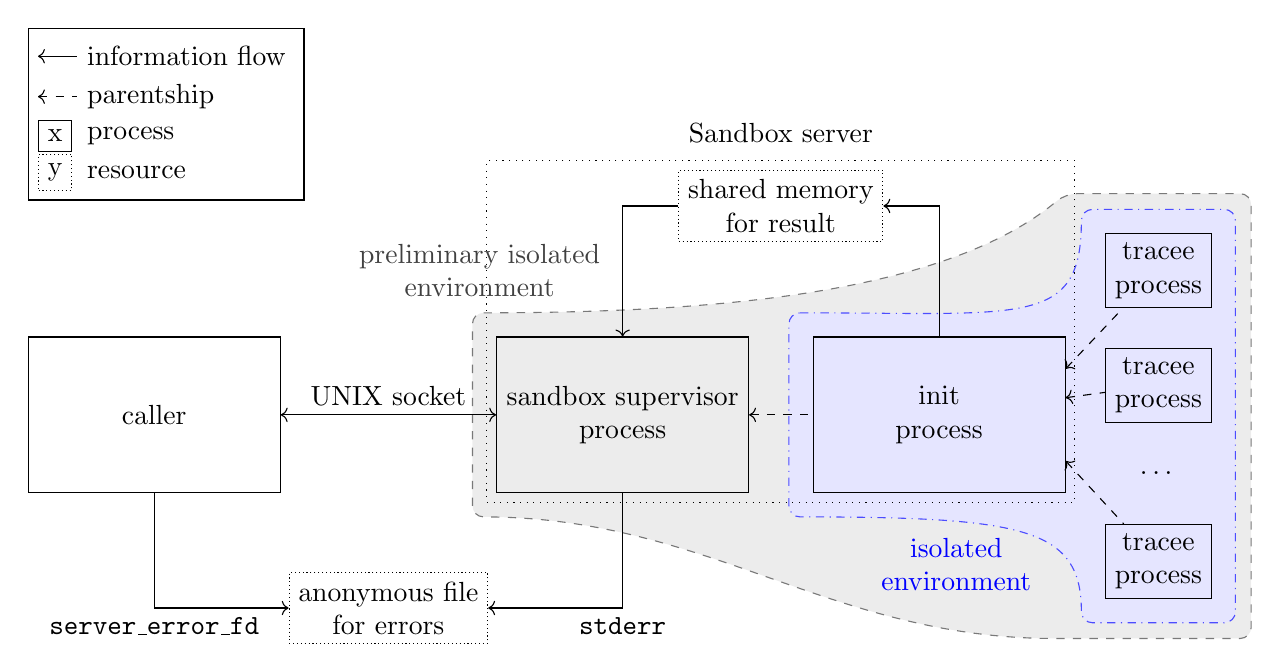
\begin{tikzpicture}[align=center]
    \node [draw, densely dotted] (errors) {anonymous file\\for errors};
    \node [draw, above left=1cm and 0.1cm of errors, minimum height=1.9777087639995352cm, minimum width=3.2cm] (caller) {caller};
    \node [draw, above right=1cm and 0.1cm of errors, minimum height=1.9777087639995352cm, minimum width=3.2cm] (supervisor) {sandbox supervisor\\process};

    \node[draw, above right=1.2cm and -0.9cm of supervisor, densely dotted] (shmem) {shared memory\\for result};
    \node [draw, below right=1.2cm and -0.9cm of shmem, minimum height=1.9777087639995352cm, minimum width=3.2cm] (init) {init\\process};

    \node [draw, above right=-0.1cm and 0.5cm of init.east] (tracee_mid) {tracee\\process};
    \node [draw, above=0.5cm of tracee_mid] (tracee_up) {tracee\\process};
    \node [below=0.5cm of tracee_mid] (tracee_dots) {\ldots};
    \node [draw, below=0.5cm of tracee_dots] (tracee_bottom) {tracee\\process};

    \draw[<->] (caller) -- node[above] {UNIX socket} (supervisor);
    \draw[->] (caller) |- node[below] {\texttt{server\_error\_fd}} (errors);
    \draw[->] (supervisor) |- node[below] {\texttt{stderr}} (errors);
    \draw[<-] (supervisor.north) |- (shmem);
    \draw[<-] (shmem) -| (init.north);
    \draw[<-, dashed] (supervisor) -- (init);
    \draw[<-, dashed] (init) -- (tracee_mid);
    \draw[<-, dashed] (init.20) -- (tracee_up);
    \draw[<-, dashed] (init.-20) -- (tracee_bottom);

    \begin{scope}[on background layer]
        \draw [dashed, rounded corners, darkgray!70, fill=darkgray!10]
            ($(supervisor.north west)+(-0.3,0.3)$) .. controls +(0:3cm) and +(220:2cm) .. node[above,inner sep=0.2cm, pos=0.01, darkgray] {preliminary isolated\\environment}
            ($(tracee_up.north west)+(-0.5,0.5)$) --
            ($(tracee_up.north east)+(0.5,0.5)$) --
            ($(tracee_bottom.south east)+(0.5,-0.5)$) --
            ($(tracee_bottom.south west)+(-0.5,-0.5)$) .. controls +(180:3cm) and +(0:3cm) ..
            ($(supervisor.south west)+(-0.3,-0.3)$) --
            cycle;
    \end{scope}

    \begin{scope}[on background layer]
        \draw [dash dot, rounded corners, blue!70, fill=blue!10]
            ($(init.north west)+(-0.3,0.3)$) .. controls +(0:3cm) and +(270:1.5cm) ..
            ($(tracee_up.north west)+(-0.3,0.3)$) --
            ($(tracee_up.north east)+(0.3,0.3)$) --
            ($(tracee_bottom.south east)+(0.3,-0.3)$) --
            ($(tracee_bottom.south west)+(-0.3,-0.3)$) .. controls +(90:1.2cm) and +(0:3cm) .. node[below,inner sep=0.2cm, pos=0.7, blue] {isolated\\environment}
            ($(init.south west)+(-0.3,-0.3)$) --
            cycle;
    \end{scope}

    \begin{scope}[on background layer]
        \node[draw, dotted, fit=(supervisor) (init) (shmem)] (server) {};
        \node[above=0.1cm of server] {Sandbox server};
    \end{scope}

    % Legend
    \matrix [draw, right] at (current bounding box.north west) {
        \draw[<-] (0,0) -- (0.5,0); & \node[right] {information flow}; \\
        \draw[<-, dashed] (0,0) -- (0.5,0); & \node[right] {parentship}; \\
        \draw node[right, draw] {x}; & \node[right] {process}; \\
        \draw node[right, draw, densely dotted] {y}; & \node[right] {resource}; \\
    };

\end{tikzpicture}
\caption{Caller requests and receives results of executing untrusted programs through UNIX socket. Sandbox server dies on error leaving the error message for the caller in an anonymous file. Sandbox server consist of the supervisor process and its child --- the init process that is spawned for each request. Init process performs role of the init process in the PID namespace of tracee processes. Init process passes errors and results to the supervisor process using shared memory. To reduce overhead of setting up the isolated environment for each request, common work is done only once to create the preliminary isolated in the supervisor process.}
\label{fig:caller_to_sandbox_server_communication}
\end{figure}

Sandbox works as a set of separate processes. Caller spawns the sandbox server, which consists of the supervisor process that for each request spawns init process that manages tracee processes of the request. A request consist of an isolated environment configuration along with the program to execute and its arguments. A separate init process is required by PID namespaces. To minimize the attack surface in case of a compromise, it is better to separate the init process from the supervisor process. Figure \ref{fig:caller_to_sandbox_server_communication} illustrates this separation.

For each request, an isolated environment needs to be prepared for the executed program. Preliminary isolated environment that is managed by sandbox supervisor process is there to reduce overhead of preparing the isolated environment during handling of the subsequent requests. Sandbox is designed for handling many subsequent requests, and setting up the isolated environment again and again requires repeating the same steps. Steps that can be done once for all requests without a security or an isolation trade-off are performed once and make up the preliminary isolated environment. One of such steps is creating a cgroup hierarchy for the init and tracee processes.

Communication is performed differently in different places. The caller sends requests and receives results via UNIX socket connected with the sandbox supervisor process. Fatal errors in the sandbox server are reported to the caller using an anonymous file for errors. This could be done over the UNIX socket but, to simplify the communication protocol it is separated. This way we do not have to deal with problematic cases like reporting error about problems with sending data over the socket --- the error would have to be reported via the problematic socket. Init process reports request results to supervisor using shared memory mapping.

The init process is the parent of the main tracee process and orphaned tracee processes as a property of PID namespaces \cite{man_pid_namespaces}. Sandbox supervisor process is the parent of the init process. Although the caller is the parent process of the sandbox supervisor process, sandbox server is implemented without this assumption. Instead of dying upon the caller process death, the sandbox supervisor watches the UNIX socket for a other-end-closure event of the connection. When this happens it exits immediately. Init process is configured to be killed as soon as the supervisor becomes dead, and trace processes will be killed by the Linux kernel when the init process dies or is killed. Therefore the sandbox server is not bound to the caller process but the UNIX socket instead.

\section{Sandbox immediate termination on connection close or supervisor death}

It is desirable to have trace processes and the sandbox terminated upon closure of the caller's end of the connection (e.g. because of death of the caller process). It is also desirable in case one of the sandbox processes dies. This is because running the tracee processes longer makes no sense as nobody will collect the result. Even more it is an unnecessary waste of the resources. Therefore sandbox terminates as soon as one of these events happens.

While the init process is handling the request, sandbox supervisor process observes with \texttt{poll()} \cite{man_poll} the socket connection to the client for closure event \texttt{POLLHUP} and the init process's PID file descriptor for \texttt{POLLIN} (which means the process become dead). This way, the supervisor process is notified immediately about the closure of the other end of the connection. Upon this event the supervisor process terminates immediately.

While the init process is not spawned, the supervisor process waits for the incoming request by blocking on \texttt{recvmsg()} \cite{man_recvmsg} on the connection, which will return 0 when the other end becomes closed. In such case, the supervisor exits immediately.

To ensure the init process does not outlive the supervisor process, it asks the kernel to kill it with \texttt{SIGKILL} when the supervisor process dies. This is done by calling \\\texttt{prctl(PR\_SET\_PDEATHSIG, SIGKILL)} \cite{man_prctl} and checking if the parent (i.e. sandbox supervisor process) is already dead after the \texttt{prctl()} call. \texttt{prctl()} is not enough by itself because if the parent process dies before the call, the process is reparented and the signal is not sent.

Checking if the parent is dead in the init process cannot be done by simply checking if \texttt{getppid()} \cite{man_getppid} returns value equal to the PID of the sandbox supervisor. This is because the init process is a member of a new PID namespace and \texttt{getppid()} returns 0, as sandbox supervisor or the parent process after reparenting is outside of this PID namespace. To deal with it, supervisor process opens a PID file descriptor on itself (via \texttt{pidfd\_open()} \cite{man_pidfd_open}) and passes it to the init process that checks with \texttt{poll()} \cite{man_poll} if it is readable. PID file descriptor becomes readable only after the process it refers to becomes dead \cite{man_pidfd_open}.

Tracee processes will be terminated by the kernel with \texttt{SIGKILL} immediately when the init process becomes dead, as it is the init process in the tracee processes' PID namespace \cite{man_pid_namespaces}.

All of the above ensures that if init process terminates, tracee process are killed and if supervisor terminates, then init process and tracee processes are terminated as well.

\section{TODO}

\section{Caller}

\section{Sandbox server}

THIS SECTION NEEDS AND WILL BE REWORED

Sandbox is spawned as a separate process and this process executes sandboxing requests e.g. execute program A with configuration B. Communication between the caller and the sandbox server process uses UNIX domain socket. Errors regarding handling a specific request are reported through the UNIX socket as a response to the sandbox request. A separate anonymous file (created using \texttt{memfd\_create()}) is used for reporting fatal errors of the sandbox server process - it fills the file with an error description and dies afterwards. Such separation allows for a simpler protocol to be used for communicating through the UNIX socket e.g. reporting errors about writing to the socket are reported using the anonymous file instead of the socket itself. Figure \ref{fig:caller_to_sandbox_server_communication} illustrates the design.


Sandbox needs to execute an untrusted executable. To do this it needs to \texttt{fork()} a child process and call \texttt{execve()} in the child process. Our use case involves executing short-running programs frequently. \texttt{fork()} syscall may take a long time \cite{redis-latency-generated-by-fork} - the bigger RSS (resident set size - RAM pages that are actually in use) the longer time \texttt{fork()} needs. To reduce \texttt{fork()} latency, the caller spawns sandbox server process that executes a separate executable -- containing only the sandbox, therefore reducing the RSS to the minimum and speeding up \texttt{fork()}. Additional benefits of this approach are setting up all common work before running executing the untrusted executable once i.e. when the sandbox server starts e.g. closing stray file descriptors not marked with \texttt{O\_CLOEXEC} flag and setting up cgroups. The only overhead is passing data and file descriptors through the UNIX socket -- from caller to the sandbox server process and back.

\section{Limiting the number of processes and threads}
TODO: cgroup

\section{Isolating filesystem}
TODO

\section{Limiting memory}
TODO: prlimit + cgroup

\section{Limiting execution time}
TODO

\section{Collecting statistics}

\subsection{Execution real time}
TODO

\subsection{Execution CPU time}
TODO

\subsection{Peek memory usage}
TODO

% \section{}

TODO NOTES:

% unshare_newpid_two_children.cc
It seems that the PID namespace init process cannot exit unless all the processes are dead and *waited* i.e. exit\_group() blocks. Here it only helps if we kill the parent. The parent of pid2 is not pid which it may seem a bit strange from inside the new namespace as there are two roots in the process hierarchy. Also init inherits orphaned children of processes inside the namespace e.g. of process pid2. So that orphaned children don't have to be adopted by an ancestor process.

RLIMIT\_CPU: limit is inherited and preserved across execve but is not shared with child processes i.e. process can spawn a child that uses up limit of X seconds, and later spawn another child that now has X seconds of cpu time, not 0 seconds.

\chapter{Evaluation} \label{chapter:evaluation}

\fi

\printbibliography

\end{document}
